\begin{theo}[Conservatieve en niet-conservatieve krachten]{Conservatieve en niet-conservatieve krachten}
    Een \textbf{conservatieve kracht} is een kracht waarbij de netto-arbeid geleverd door deze kracht nul is bij een gesloten baan, onafhankelijk is van de afgelegde weg. Bijvoorbeeld: 
    \begin{itemize}
        \item de gravitatiekracht: $ \Vec{F}_g = m\Vec{g} $      
        % \\
        % \begin{minipage}{.48\textwidth}
        %     \vspace*{\fill}
        %     \begin{align*}
        %         W &= -\int_a^b mg\hat{k}d\Vec{r} \\
        %           &= -mg\int_a^b\hat{k}(dx\hat{i}+dy\hat{j}+dz\hat{k}) \\
        %           &= -mg\int_a^bdz \\
        %           &= -mg(z_b - z_a)
        %     \end{align*}
        %     \vspace*{\fill}
            
        % \end{minipage} 
        % \begin{minipage}{.25\textwidth}
        
        %     \centering
        %     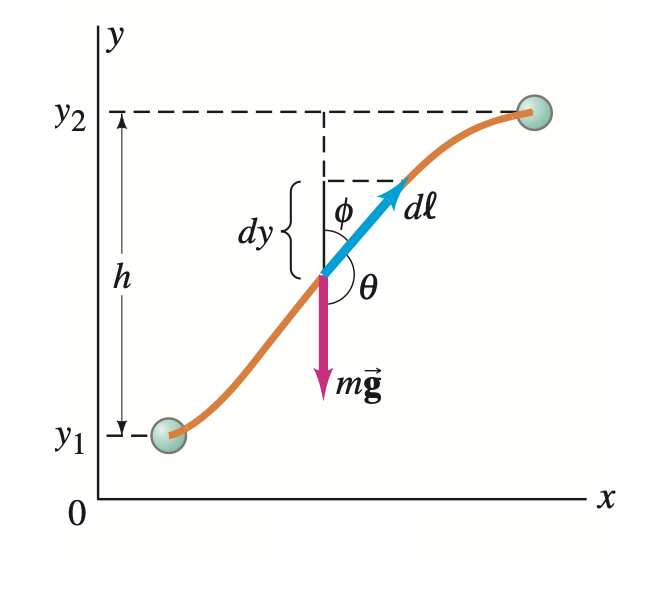
\includegraphics[scale = 0.225]{Images/Dynamica/ConservatieveZwaartekracht.png}
            
        % \end{minipage}
        \item de veerkracht: $ \Vec{F}_s = -k\Vec{x} $
    \end{itemize}
    
    \noindent Een \textbf{niet-conservatieve kracht} is een kracht waarbij de netto-arbeid geleverd door deze kracht afhankelijk is van de gevolgde weg 
    % \\ \\
    % \begin{minipage}{.44 \textwidth}
    %         \noindent\fbox{\parbox{\textwidth}{
    %         A crate is pushed slowly at constant speed across a rough floor
    %         from position 1 to position 2 via two paths: one straight and one curved. The pushing force $ F_P $ is in the direction of motion at each point. (The friction force opposes the motion.) Hence for a constant magnitude pushing force, the work it does is $ W = F_Pd$ , so if $ d $ is greater (as for the curved path), then $ W $  is greater. The work done does not depend only on points 1 and 2; it also depends on the path taken.}}       
    % \end{minipage} 
    % \begin{minipage}{.54\textwidth}
    %     \centering
    %     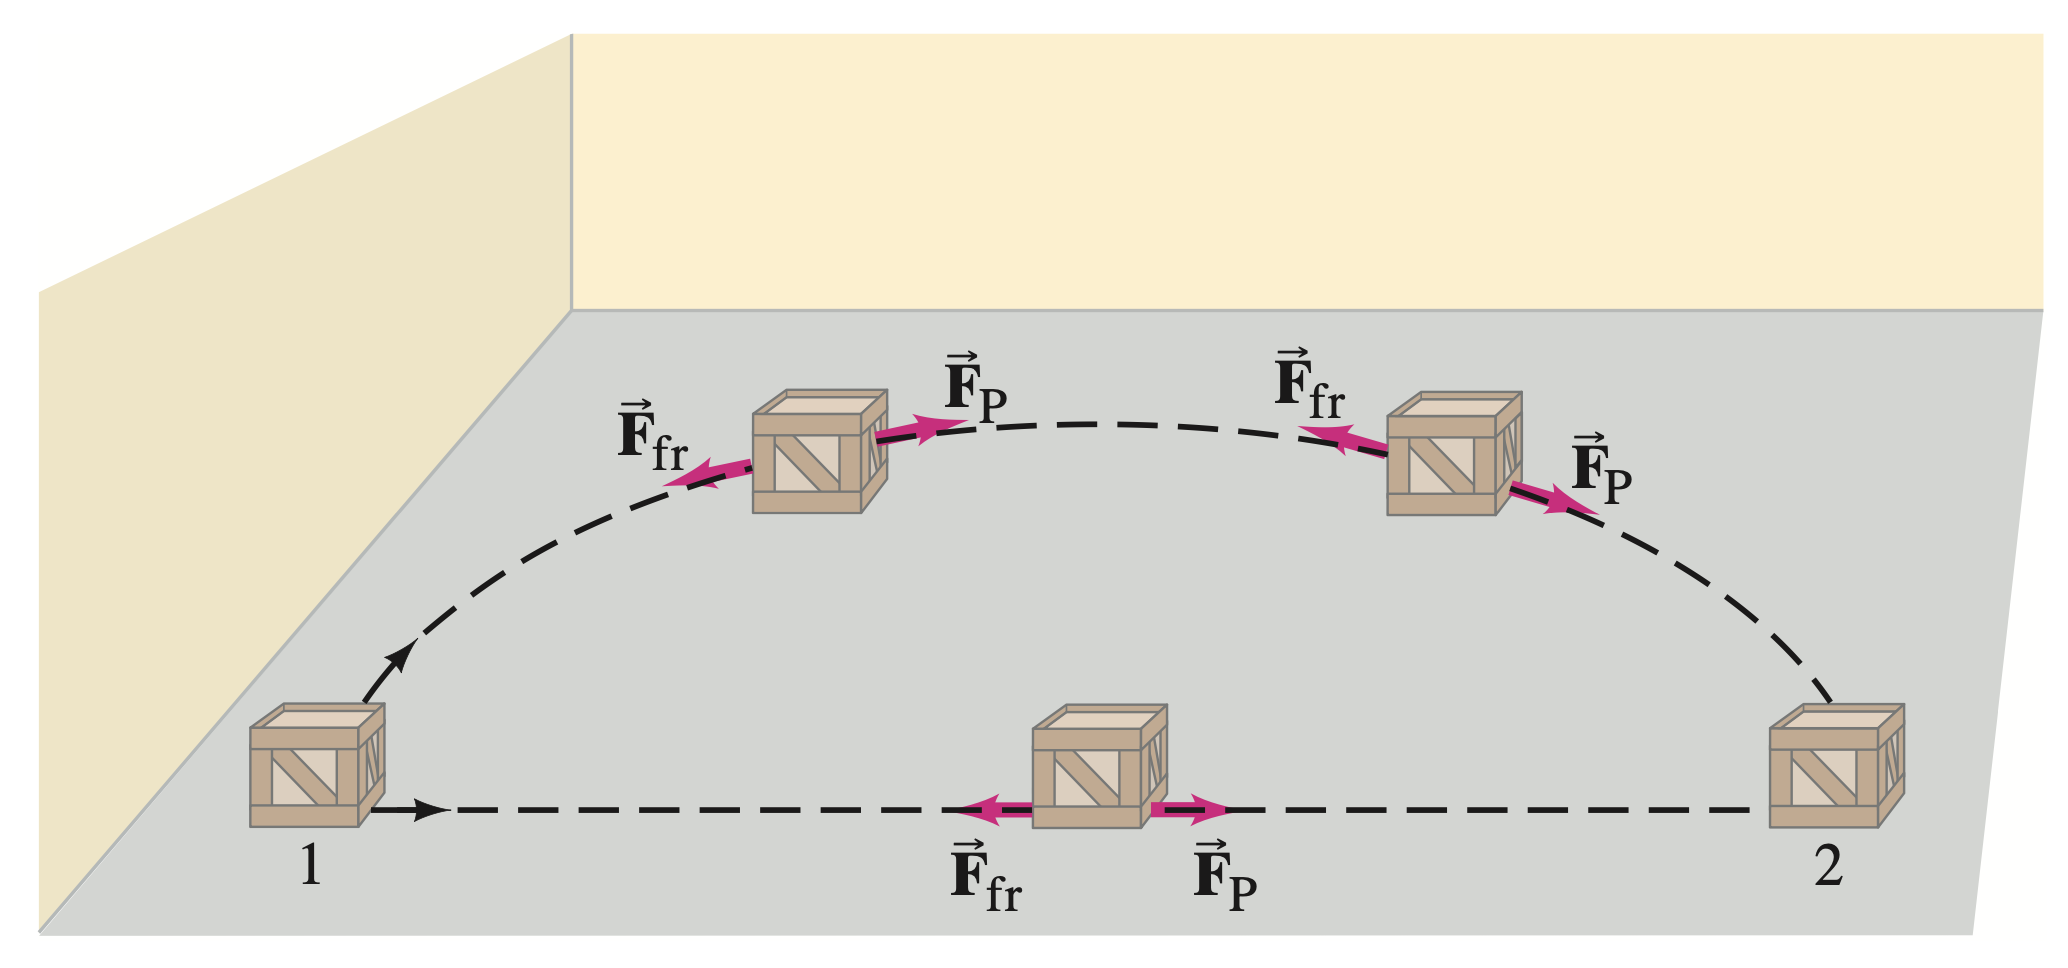
\includegraphics[scale = 0.2]{Images/Dynamica/NietConservatief.png}
    % \end{minipage}
\end{theo}

% \begin{theo}[Niet-conservatieve kracht]{Niet-conservatieve kracht}
%     Een \textbf{niet-conservatieve kracht} is een kracht waarbij de netto-arbeid geleverd door deze kracht afhankelijk is van de gevolgde weg \\ \\
%         \begin{minipage}{.44 \textwidth}
%                 \noindent\fbox{\parbox{\textwidth}{
%                 A crate is pushed slowly at constant speed across a rough floor
%                 from position 1 to position 2 via two paths: one straight and one curved. The pushing force $ F_P $ is in the direction of motion at each point. (The friction force opposes the motion.) Hence for a constant magnitude pushing force, the work it does is $ W = F_Pd$ , so if $ d $ is greater (as for the curved path), then $ W $  is greater. The work done does not depend only on points 1 and 2; it also depends on the path taken.}}       
%         \end{minipage} 
%         \begin{minipage}{.54\textwidth}
%             \centering
%             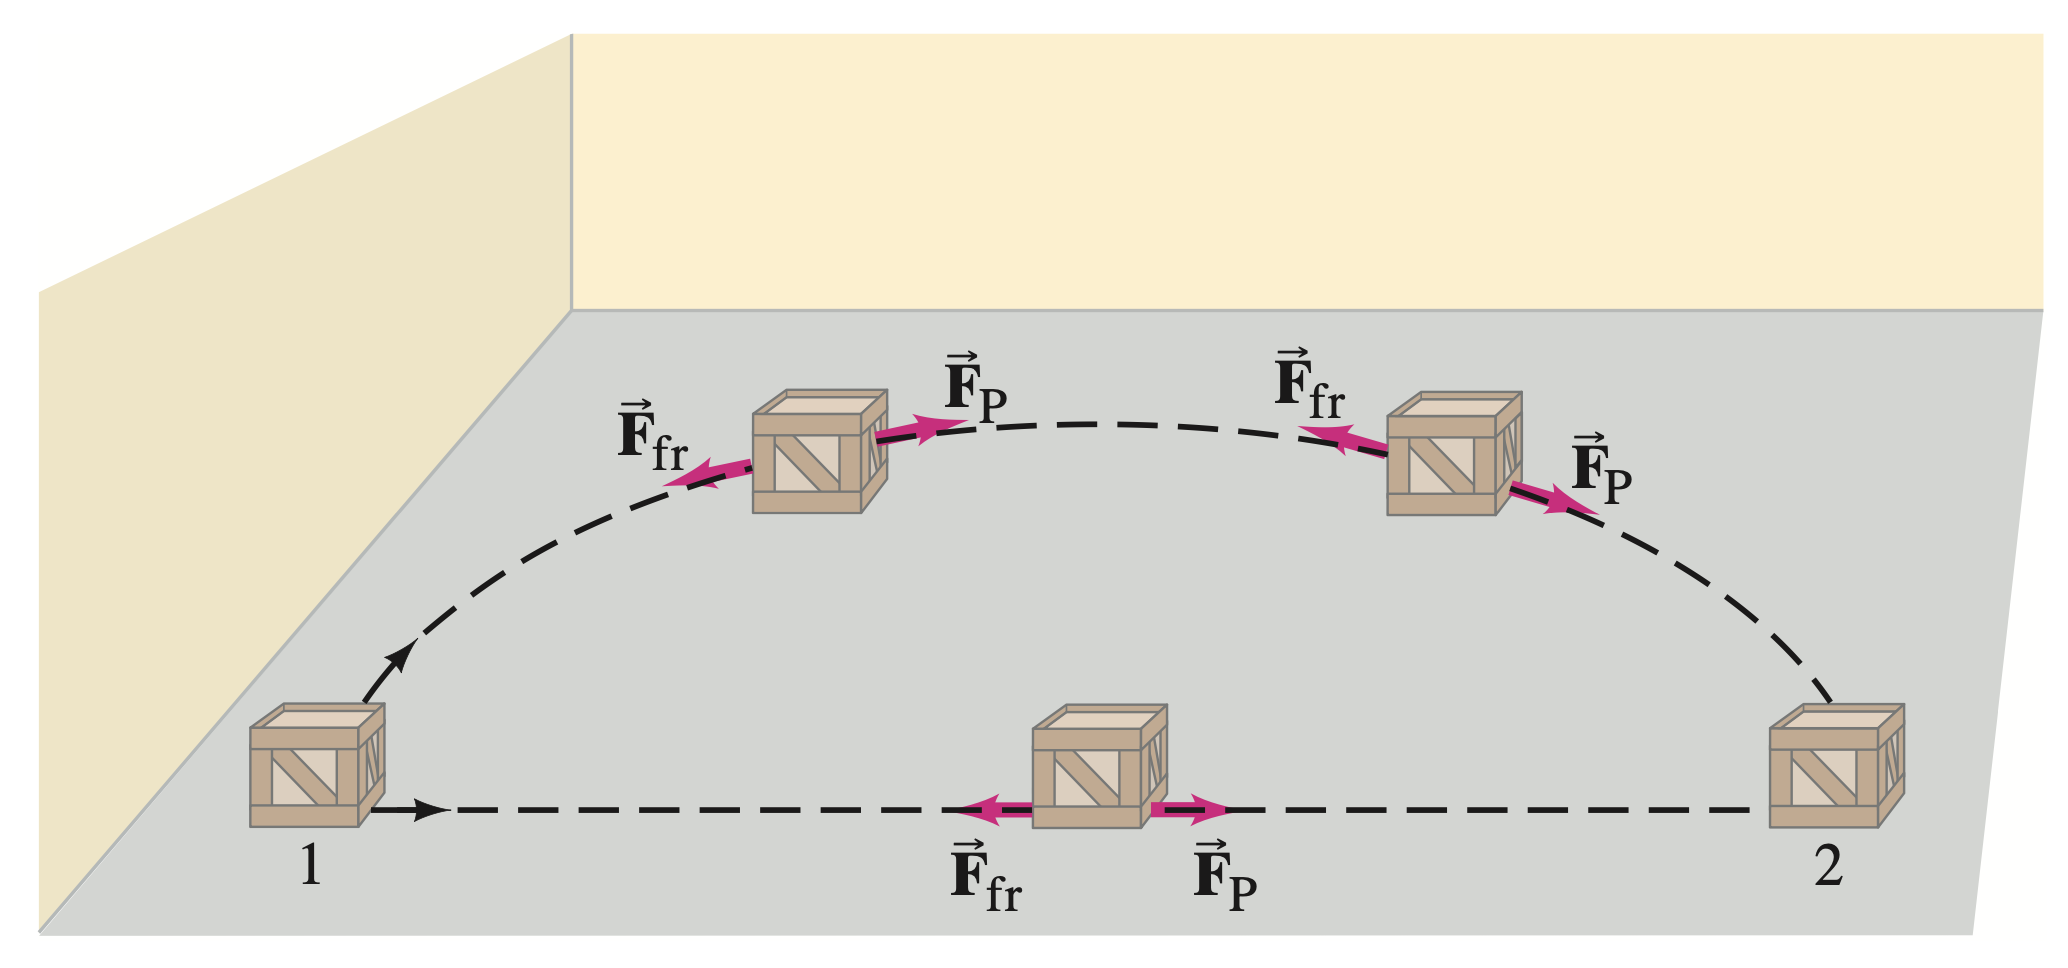
\includegraphics[scale = 0.2]{Images/Dynamica/NietConservatief.png}
%         \end{minipage}
% \end{theo}

\begin{theo}[Potentiële energie]{Potentiële energie}
    
    % Vanaf dit deelhoofdstuk spreken we ook van \textbf{potentiele energie} $ U $, wat geassocieerd wordt met krachten die afhangen van positie of afhangen van omgeving, dus: conservatieve krachten. \\
    
    \noindent De arbeid geleverd door een conservatieve kracht is gelijk aan het tegengestelde van de verandering in potentiële energie: 
        \begin{equation*}
            \Delta U = U_2 - U_1 = \int_1^2dU = -\int_1^2 \Vec{F}\cdot d\Vec{r} = -W
        \end{equation*}
    
    \noindent Het is belangrijk om aan te halen dat het \textbf{verschil} in potentiële energie onafhankelijk is van het referentiestelsel. Hierdoor kunnen we de volgende redenering maken:
    \begin{align*}
        \hspace{4.5cm} U(\Vec{r}) - U(\Vec{r}_1) &=  -\int_{\Vec{r}_1}^{\Vec{r}} \Vec{F}\cdot d\Vec{r} \quad \quad (meestal \ kiezen \ we \  U_1 = 0) \\
            -dU &= \Vec{F}\cdot d\Vec{r}  \\
                % &= F_Tdr \\
                &= drFcos(\theta) 
    \end{align*}
    Uit deze berekeningen kunnen we een belangrijke formule halen:
    \begin{equation*}
        F_T = Fcos(\theta) = -\dfrac{dU}{dr}
    \end{equation*}
    We kunnen deze vondst veralgemenen naar de 3 dimensies:
    \begin{equation*}
        \Vec{F} = -\nabla U = -\tfrac{\theta}{\theta x}U\hat{i} - \tfrac{\theta}{\theta y}U\hat{j} - \tfrac{\theta}{\theta z}U\hat{k}
    \end{equation*}
    
\end{theo}

\begin{lem}[Behoud van energie]{Bbehoud van energie}

    De wet van behoud van energie stelt dat energie niet kan worden gecreëerd of vernietigd - alleen omgezet van de ene vorm van energie in een andere. In formulevorm:
    
    \begin{equation*}
        \Delta K + \Delta U = W_{nc} 
    \end{equation*}
    \vspace{-0.5cm}
\end{lem}

\newpage

\begin{lem}[Behoud van mechanische energie]{Behoud van mechanische energie}
    We bundelen even wat vondsten van hiervoor samen:
    \begin{align*}
        K_b - K_a &= -(U_b - U_a) = U_a - U_b \\
        K_a + U_a &= K_b + U_b \\ 
        E_a = (K + U)_a &= (K + U)_b = E_b
    \end{align*}
    
    \noindent We zien nu dus dat de totale mechanische energie $ E = K + U $ van een deeltje constant blijft ($ E_a = E_b $) als de inwerkende krachten die arbeid leveren conservatief zijn. In formulevorm:
    
    \begin{equation*}
        \Delta E = \Delta K + \Delta U = 0
    \end{equation*}
    \vspace{-0.5cm}
\end{lem}

% \begin{app}[Arbeid geleverd door een veer]{Arbeid geleverd door een veer}

%     We berekenen het verschil in potentiele energie van $ 0 \to x $ met x positief of negatief:
    
%     \begin{align*}
%         \Delta U = U(x) - U(0) = -\int_0^x (-kx)dx = \dfrac{1}{2}kx^2 = - W_s
%     \end{align*}
    
%     \noindent De mechanische energie blijft constant als de inwerkende krachten conservatief zijn, wat natuurlijk zo is bij een veer. We bekomen de volgende formule indien we zeggen dat $ U = U(x) $:
    
%     \begin{equation*}
%         \dfrac{1}{2}mv^2_1 + \dfrac{1}{2}kx^2_1 = \dfrac{1}{2}mv^2_2  + \dfrac{1}{2}kx^2_2
%     \end{equation*}
% \end{app}

\begin{theo}[Vermogen]{Vermogen}
    Het \textbf{vermogen} is een scalaire grootheid voor arbeid per tijdseenheid, uitgedrukt in Watt.
    \begin{itemize}
        \item \textbf{Gemiddelde:} $ P_{gem} = \dfrac{W}{\Delta t} $ 
        \item \textbf{Ogenblikkelijke:} $ P = \dfrac{dW}{dt} = \dfrac{dE}{dt} $, want arbeid = energie transformatie! \\
        We krijgen uit de definitie van arbeid: $ P = \Vec{F} \cdot \dfrac{d\Vec{r}}{dt} = \Vec{F} \cdot \Vec{v} $
    \end{itemize}
\end{theo}